% Drawing 156-7/05-1 -- folder 156-7, batch 05, archive page 81 (PDF page 82).
% Transcription: dessin : un fuseau fermé, deux arcs joignant un point marqué $0$ à gauche à un point marqué $1$ à droite ; une croix $x$ sur l'arc supérieur ; à côté, « (\uncertain{saisons} \ill{}) » ; sous le dessin, « (un \ill{} $x$ de $]0,1[$) »
% Kind: spindle (two-strand string). Method 2 (schematic redraw from the facsimile). Status: partial.
% Notes: Closed spindle: two arcs from the point 0 (left) to the point 1 (right), a cross x on the upper arc. The legend under the drawing is written as the transcription reads it; the legend on the right ("(saisons ...)") and the oblique marginal note joined to x are left out (partly illegible).
% Coordinates: 1 unit = 1 mm = 1/100 of the crop width (bbox in page fractions: [0.3, 0.72, 0.7, 0.82]).
% Redrawn by Claude (claude-opus-5-5), issue #73, 2026-11-07; not checked by a human; not compiled (no TeX in the session).
% Rights: reproduces part of the work -- behind RENDER_TRANSCRIPTS, never published by itself.
\documentclass[tikz,border=3pt]{standalone}
\usepackage{amsmath,amssymb}
\usetikzlibrary{patterns,arrows.meta}
\tikzset{pencil/.style={black!45}, struck/.style={black!35}, mark/.style={circle,draw,inner sep=1.3pt}, pt/.style={circle,fill,inner sep=0.9pt}, opt/.style={circle,draw,fill=white,inner sep=1.1pt}}
\begin{document}
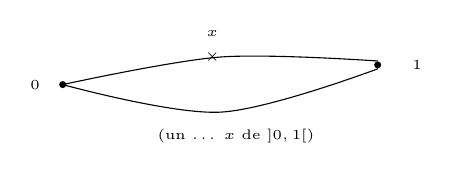
\begin{tikzpicture}[x=1mm,y=1mm,line cap=round,line join=round,font=\scriptsize]
\draw plot[smooth, tension=0.55] coordinates {(20,-19) (40,-15.5) (60,-16)};
\draw plot[smooth, tension=0.55] coordinates {(20,-19) (40,-22.5) (60,-17)};
\node[pt] at (20,-19) {};
\node[pt] at (60,-16.5) {};
\node[inner sep=1pt] at (16.5,-19) {\tiny $0$};
\node[inner sep=1pt] at (65,-16.5) {\tiny $1$};
\node[inner sep=1pt] at (39,-15.5) {\tiny $\times$};
\node[inner sep=1pt] at (39,-12.5) {\tiny $x$};
\node[inner sep=1pt] at (42,-25.5) {\tiny (un \ldots\ $x$ de $]0,1[$)};
\end{tikzpicture}
\end{document}
